\documentclass{article}

\usepackage{graphicx}
\usepackage{tikz}
\usepackage{tikzsymbols}
\usetikzlibrary{calc,patterns,shapes.geometric}
\pagestyle{empty}
\usepackage[margin=0pt]{geometry}
\geometry{papersize={14in,12in}}

\def\centerarc[#1](#2)(#3:#4:#5){\draw[#1] ($(#2)+({#5*cos(#3)},{#5*sin(#3)})$) arc (#3:#4:#5);}

\begin{document}
	\begin{figure}
		\centering
		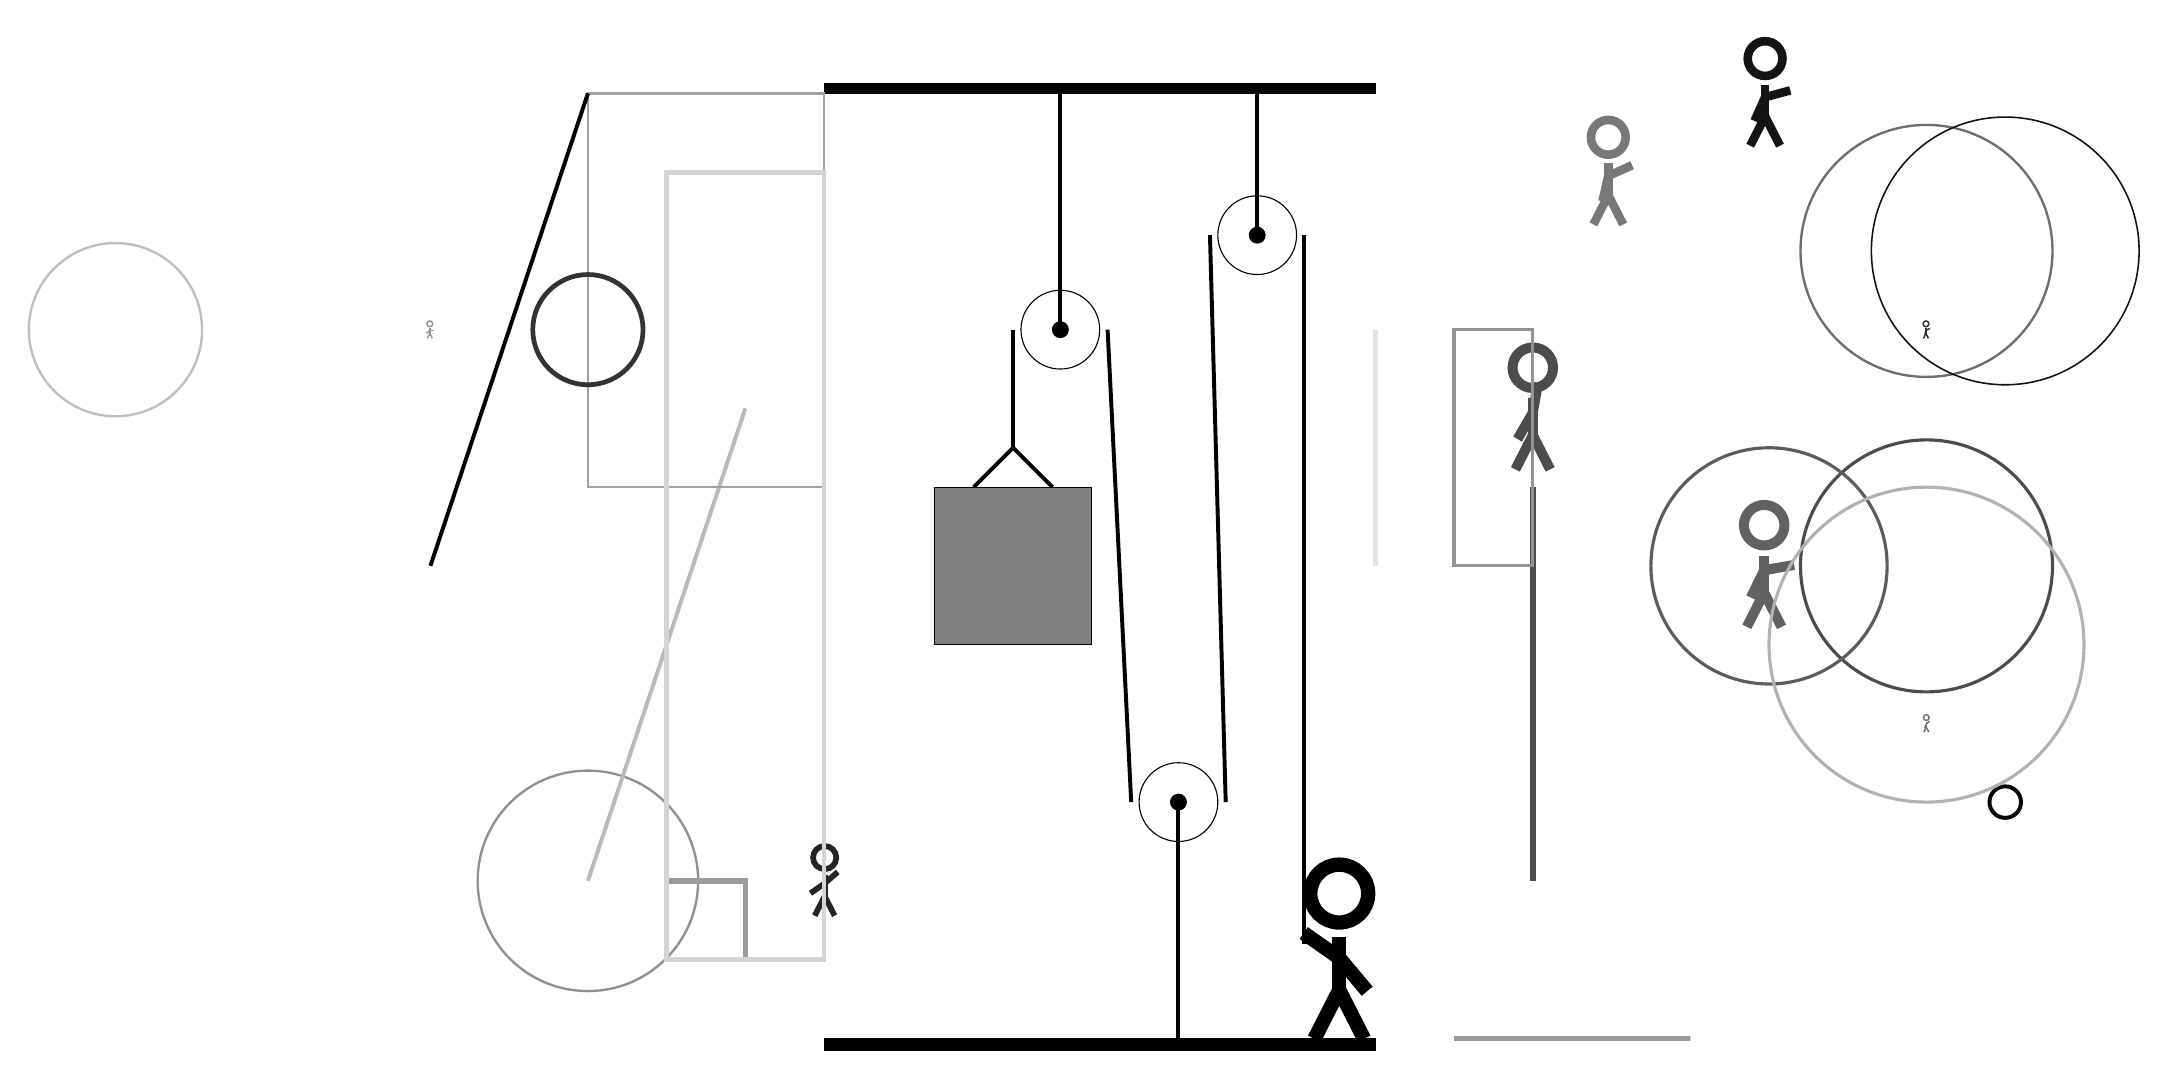
\begin{tikzpicture}
			%%%%% START %%%%%
			
			\draw[fill=black] (-2, 9) rectangle (5, 9.125);
			
			\draw (1, 6) circle (0.5);
			\draw[fill=black] (1, 6) circle (0.1);
			\draw[line width=0.5mm]  (1, 9) -- (1, 6);
			
			\draw[fill=white](2.5, 0) circle (0.5);
			\draw[fill=black] (2.5, 0) circle (0.1);
			\draw[line width=0.5mm]  (2.5, -3) -- (2.5, 0);
			
			\draw[fill=white](3.5, 7.2) circle (0.5);
			\draw[fill=black] (3.5, 7.2) circle (0.1);
			\draw[line width=0.5mm] (3.5, 9) -- (3.5, 7.2);
			
			\draw[line width=0.7mm, color=black!70] (7, 4) rectangle (7, -1);
			
			\draw[line width=0.7mm, color=black!11] (5, 6) rectangle (5, 3);
			\draw [line width=0.3mm, color=black!57](12, 7) circle (1.6);
			\node[line width=0.3mm, color=black!43] at (-7, 6) {\Strichmaxerl[1][43][0]};
			\node[line width=0.7mm, color=black!70] at (7, 5) {\Strichmaxerl[7][60][80]};
			\draw [line width=0.4mm, color=black!70](12, 3) circle (1.6);
			\node[line width=0.6mm, color=black!82] at (12, 6) {\Strichmaxerl[1][76][24]};
			
			\draw [line width=0.3mm, color=black!43](-5, -1) circle (1.4);
			\draw[line width=0.5mm, color=black!27](-5, -1) -- (-3, 5);
			\node[line width=0.3mm, color=black!62] at (10, 3) {\Strichmaxerl[7][64][10]};
			\draw[line width=0.6mm, color=black!40] (6, -3) rectangle (9, -3);
			
			\draw [line width=0.2mm, color=black!93](13, 7) circle (1.7);
			\node[line width=0.3mm, color=black!92] at (10, 9) {\Strichmaxerl[6][66][15]};
			
			\node[line width=0.6mm, color=black!86] at (-2, -1) {\Strichmaxerl[4][35][41]};
			\draw [line width=0.5mm, color=black!98](13, 0) circle (0.2);
			\draw [line width=0.4mm, color=black!64](10, 3) circle (1.5);
			\draw[line width=0.7mm, color=black!39] (-4, -2) rectangle (-3, -1);
			\draw[line width=0.3mm, color=black!37] (-2, 4) rectangle (-5, 9);
			\draw[line width=0.4mm, color=black!42] (6, 3) rectangle (7, 6);
			\draw [line width=0.6mm, color=black!80](-5, 6) circle (0.7);
			\draw[line width=0.6mm, color=black!17] (-2, 8) rectangle (-4, -2);
			
			\draw[line width=0.5mm, color=black!100](-5, 9) -- (-7, 3);
			
			\draw [line width=0.4mm, color=black!30](12, 2) circle (2.0);
			\draw [line width=0.3mm, color=black!25](-11, 6) circle (1.1);
			\node[line width=0.4mm, color=black!53] at (8, 8) {\Strichmaxerl[6][77][24]};
			\node[line width=0.6mm, color=black!56] at (12, 1) {\Strichmaxerl[1][69][41]};
			
			\draw[line width=0.5mm] (-0.1, 4.0) -- (0.4, 4.5) -- (0.9, 4.0);
			\draw[fill=black!50] (-0.6, 4.0) rectangle (1.4, 2.0);
			
			\draw[line width=0.5mm] (0.4, 6) -- (0.4, 4.5);
			\centerarc[line width=0.5mm](1, 6)(0:180:0.6);
			\draw[line width=0.5mm](1.6, 6) -- (1.9, 0);
			\centerarc[line width=0.5mm](2.5, 0)(180:360:0.6);
			\draw[line width=0.5mm](3.1, 0) -- (2.9, 7.2);
			\centerarc[line width=0.5mm](3.5, 7.2)(0:180:0.6);
			\draw[line width=0.5mm](4.1, 7.2) -- (4.1, -1.8);
			
			\node at (4.5, -1.9) {\Strichmaxerl[10][-35][-50]};
			
			\draw[fill=black] (-2, -3) rectangle (5, -3.15);
			
			%%%%% END %%%%%
		\end{tikzpicture}
	\end{figure}	
\end{document}